%% %% %% %%
%%
%% Parte A de la práctica
%%
%% %% %% %%

\documentclass[../procedimientos.tex]{subfiles}
\graphicspath{{\subfix{../../images/}}}

\begin{document}
\clearpage
\subsection{Parte A}
\subsubsection{Instrucciones}
Implantar las siguientes funciones:
\begin{itemize}
  \item $f_1 (abc) = a\nt{b}c + \nt{a}$
  \item $f_2 (abc) = ab + \nt{b}a\nt{c} + a \odot c$
  \item $f_3 (abc) = (a + \nt{b} + \nt{c}) (b + c)$
\end{itemize}

\subsubsection{Análisis}
Antes de comenzar a implementar la solución en \textit{Quartus}, es importante 
deducir el comportamiento esperado, con la finalidad de detectar errores en el 
funcionamiento. Para realizar esto, haremos uso de las tablas de verdad de las 
expresiones.

Para el caso de las función $f_1(abc)$, se tiene la siguiente tabla de verdad:
\begin{table}[H]
  \centering
  \begin{tabular}{ccc|cc|c}
    \hline
    $a$ & $b$ & $c$ & $a\nt{b}c$ & $\nt{a}$ & $f_1$\\
    \hline
    0 & 0 & 0 & 0 & 1 & 1\\
    0 & 0 & 1 & 0 & 1 & 1\\
    0 & 1 & 0 & 0 & 1 & 1\\
    0 & 1 & 1 & 0 & 1 & 1\\
    1 & 0 & 0 & 0 & 0 & 0\\
    1 & 0 & 1 & 1 & 0 & 1\\
    1 & 1 & 0 & 0 & 0 & 0\\
    1 & 1 & 1 & 0 & 0 & 0\\
    \hline
  \end{tabular}
  \caption{Tabla de verdad de $f_1(abc)$ (Parte A)}
  \label{tab:a_f1}
\end{table}

Para el caso de la función $f_2(abc)$, es un poco más cómodo hacer una 
representación a través de la forma equivalente de la compuerta XNOR, 
recordando que esta tiene más precedencia que la compuerta AND u OR, por lo 
que queda representada de la siguiente forma:
$$f_2(abc) = ab + \nt{b}a\nt{c} + ac + \nt{a}\nt{c}$$
Entonces, la tabla de verdad queda representada de la siguiente forma:
\begin{table}[H]
  \centering
  \begin{tabular}{ccc|cccc|c}
    \hline
    $a$ & $b$ & $c$ & $ab$ & $\nt{b}a\nt{c}$ & $ac$ & $\nt{a}\nt{c}$ & $f_2$\\
    \hline
    0 & 0 & 0 & 0 & 0 & 0 & 1 & 1\\
    0 & 0 & 1 & 0 & 0 & 0 & 0 & 0\\
    0 & 1 & 0 & 0 & 0 & 0 & 1 & 1\\
    0 & 1 & 1 & 0 & 0 & 0 & 0 & 0\\
    1 & 0 & 0 & 0 & 1 & 0 & 0 & 1\\
    1 & 0 & 1 & 0 & 0 & 1 & 0 & 1\\
    1 & 1 & 0 & 1 & 0 & 0 & 0 & 1\\
    1 & 1 & 1 & 1 & 0 & 1 & 0 & 1\\
    \hline
  \end{tabular}
  \caption{Tabla de verdad de $f_2(abc)$ (Parte A)}
  \label{tab:a_f2}
\end{table}

Prosiguiendo con la obtención de las tablas de verdad, se tiene la la tabla de 
verdad de la función lógica $f_3(abc)$, para la cual se tiene lo siguiente:
\begin{table}[H]
  \centering
  \begin{tabular}{ccc|cc|c}
    \hline
    $a$ & $b$ & $c$ & $a + \nt{b} + \nt{c}$ & $b + c$ & $f_3$\\
    \hline
    0 & 0 & 0 & 1 & 0 & 0\\
    0 & 0 & 1 & 1 & 1 & 1\\
    0 & 1 & 0 & 1 & 1 & 1\\
    0 & 1 & 1 & 0 & 1 & 0\\
    1 & 0 & 0 & 1 & 0 & 0\\
    1 & 0 & 1 & 1 & 1 & 1\\
    1 & 1 & 0 & 1 & 1 & 1\\
    1 & 1 & 1 & 1 & 1 & 1\\
    \hline
  \end{tabular}
  \caption{Tabla de verdad de $f_3(abc)$ (Parte A)}
  \label{tab:a_f3}
\end{table}

Combinando los resultados de la Tablas \ref{tab:a_f1}, \ref{tab:a_f2} y 
\ref{tab:a_f3}, se tiene lo siguiente:
\begin{table}[H]
  \centering
  \begin{tabular}{ccc|ccc|c}
    \hline
    $a$ & $b$ & $c$ & $f_1$ & $f_2$ & $f_3$ & HEX\\
    \hline
    0 & 0 & 0 & 1 & 1 & 0 & 6\\
    0 & 0 & 1 & 1 & 0 & 1 & 5\\
    0 & 1 & 0 & 1 & 1 & 1 & 7\\
    0 & 1 & 1 & 1 & 0 & 0 & 4\\
    1 & 0 & 0 & 0 & 1 & 0 & 2\\
    1 & 0 & 1 & 1 & 1 & 1 & 7\\
    1 & 1 & 0 & 0 & 1 & 1 & 3\\
    1 & 1 & 1 & 0 & 1 & 1 & 3\\
    \hline
  \end{tabular}
  \caption{Resumen del comportamiento de $f_1$, $f_2$ y $f_3$ (Parte A)}
  \label{tab:a_summary}
\end{table}

\subsubsection{Implementación en Quartus}
Para la implementación de estas compuertas en \textit{Quartus}, se creó un 
diagrama de bloques para cada una de ellas, tal como se muestra a 
continuación:
\begin{figure}[H]
  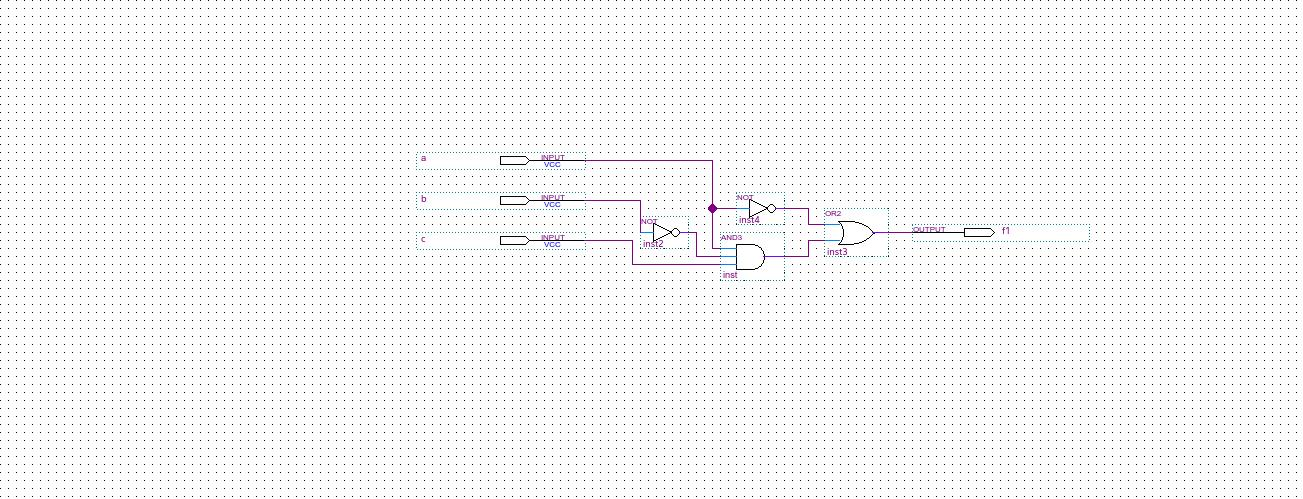
\includegraphics[width=\textwidth]{ejercicio_a1}
  \caption{Implementación de $f_1(abc)$ (Parte A)}
  \label{fig:a_f1}
\end{figure}
\begin{figure}[H]
  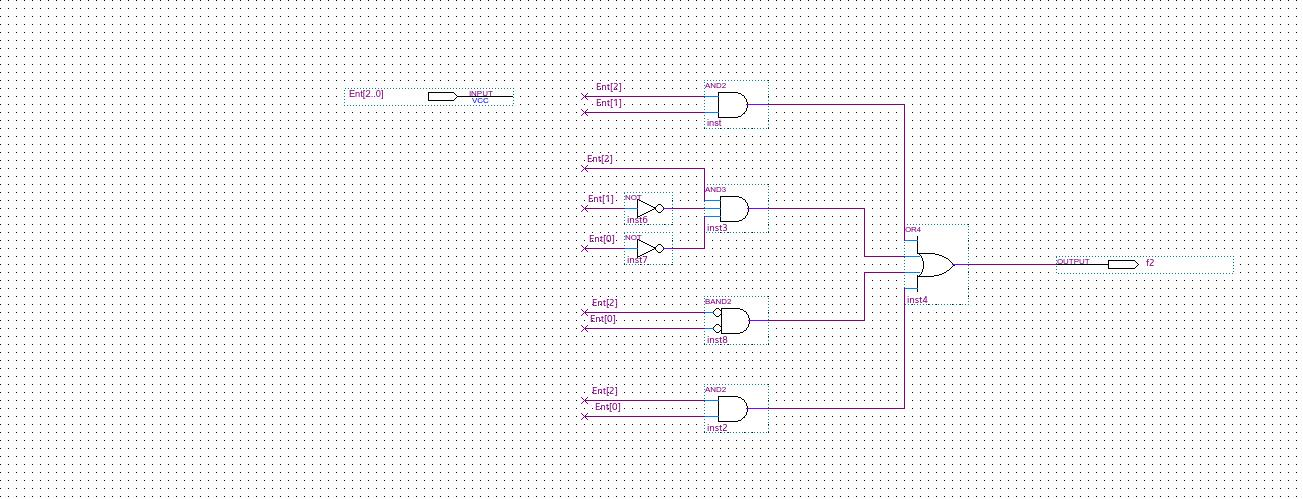
\includegraphics[width=\textwidth]{ejercicio_a2}
  \caption{Implementación de $f_2(abc)$ (Parte A)}
  \label{fig:a_f2}
\end{figure}
\begin{figure}[H]
  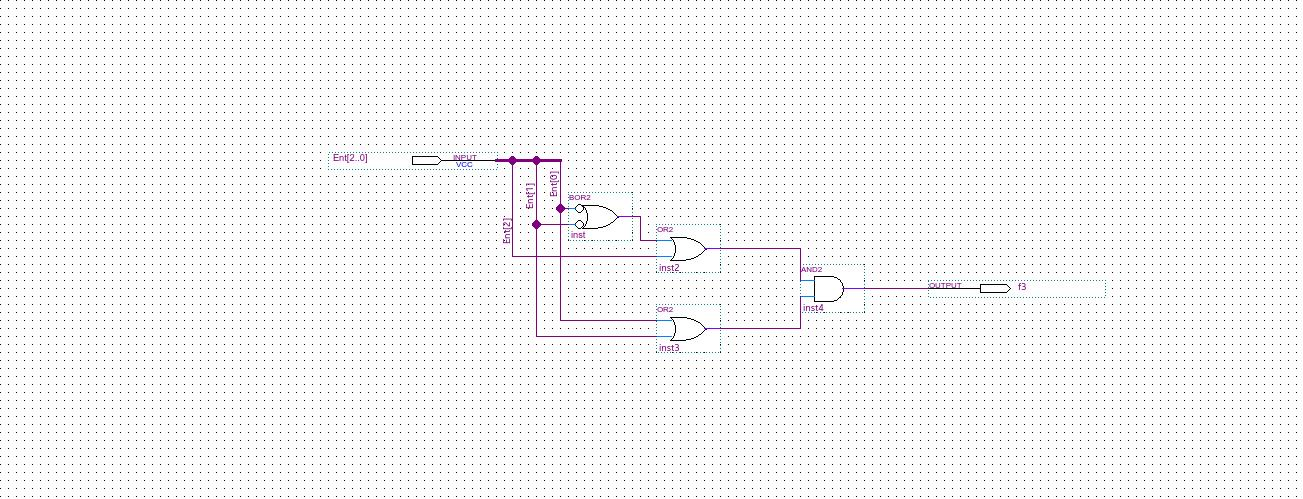
\includegraphics[width=\textwidth]{ejercicio_a3}
  \caption{Implementación de $f_3(abc)$ (Parte A)}
  \label{fig:a_f3}
\end{figure}

Tal como se puede apreciar en la Figura \ref{fig:a_f1}, las entradas se 
manejaron como valores independientes ($a$, $b$ y $c$). Una aproximación 
bastante similar a la que se tuvo en la práctica anterior.

Por otro lado, en las Figuras \ref{fig:a_f2} y \ref{fig:a_f3} se hizo uso de 
dos conceptos nuevos:
\begin{enumerate}
  \item Por una parte, los valores de $a$, $b$ y $c$ se agruparon a través 
    de una variable de tipo \textit{array} con una longitud de \textbf{tres 
    elmentos}, en la que se tiene la siguiete estructura:
    \begin{itemize}
      \item $a$ = $Ent[2]$
      \item $b$ = $Ent[1]$
      \item $c$ = $Ent[0]$
    \end{itemize}
  \item Y por el otro, se manejó un alambrado a través de etiquetas en los 
    cables, con la finalidad de evitar cruces inesperados cuando las 
    conexiones se vuelve más complicadas. Además, cuando se quiere pasar de un 
    cable que trae consigue muchas señales (como el caso de las señales de 
    arreglos) y se quiere pasar a un cable con una señal, es obligatorio poner 
    el elemento exacto del cual se tomará el valor.
\end{enumerate}

Para comprobar el comportamiento de estas funciones lógicas, se tuvo que 
implementar un apartado especial (haciendo uso de los símbolos creados 
anteriormente para cada una de las funciones) en un archivo especial. Se 
configuró la entrada como un arreglo de tres elementos y la salida también se 
implementó como otro arreglo, tal como se muestra a continuación:
\begin{enumerate}
  \item \textbf{Ent}: El arreglo de valores de entrada
    \begin{itemize}
      \item $a$ = $Ent[2]$
      \item $b$ = $Ent[1]$
      \item $c$ = $Ent[0]$
    \end{itemize}
  \item \textbf{Sal}: El arreglo de valores de salida
    \begin{itemize}
      \item $f_1$ = $Sal[2]$
      \item $f_2$ = $Sal[1]$
      \item $f_3$ = $Sal[0]$
    \end{itemize}
\end{enumerate}

Con lo anterior, es posible realizar la simulación con ayuda de un archivo de 
tipo \textit{University Program VWF}. Se configuraron las señales a 
visualizar, y se configuraron para tener las entradas mostradas en la Tabla 
\ref{tab:a_summary}. Su utilizó la \textit{Funcional Simuation}, y el resultdo 
fue el siguiente:
\begin{figure}[H]
  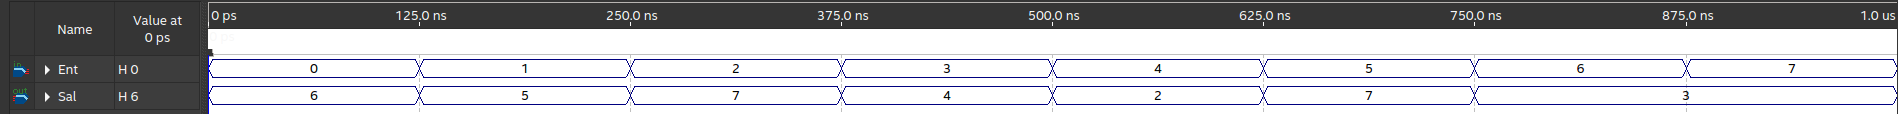
\includegraphics[width=\textwidth]{ejercicio_a_sim}
  \caption{Simulación (Parte A)}
  \label{fig:a_sim}
\end{figure}

Tal como se puede ver en la Figura \ref{fig:a_sim}, los resultados de la 
simulación fueron los mismos que los pre-calculados en la Tabla 
\ref{tab:a_summary}.

\end{document}

